\documentclass[12pt]{article}
	\usepackage{geometry}
	\geometry{margin=1in}

	\usepackage[utf8]{inputenc}
	\usepackage{graphicx}
	\graphicspath{{Include/}}
	
	\usepackage{amsmath, amssymb, mathrsfs}
	\usepackage[backend=bibtex,style=numeric]{biblatex}
	\addbibresource{./Include/bibliografia.bib}
	
	\usepackage{algorithm, algpseudocode, listings}
	\usepackage{hyperref}

	
	\title
		{
		% \vspace{-30mm}\begin{figure}[h]
		% \centering
		% 
\includegraphics[width=2in]{./Include/logo_polimi.png}
		% \end{figure}
		Anderson Acceleration for Fixed-Point Iterations
		}
		
	\author{Martino Ischia\\ \footnotesize{Supervisor: Prof. Formaggia}}
	\date{January 2021}
		
		
	\begin{document}
		\maketitle
		\begin{abstract}
			\noindent The goal of this project is twofold.\\
			Firstly, develop a C++ interface for accelerating a converging sequence of vectors.
			It should be at the same time open for extensions, in case the user wants to implement its own algorithm,
			and efficient in the solution of large systems.\\
			Secondly, making use of said interface to implement Anderson acceleration strategy and apply it on
			linear and nonlinear problems arising from the discretization of differential equations.\\
			The reader not interested in the C++ implementation can safely skip section \ref{sec:C++}, even though
			the classes described there are sometimes mentioned in section \ref{sec:app}.
		\end{abstract}
		\tableofcontents
		\pagebreak
		
		
		\section{Introduction}
			A fixed-point problem consists in finding the point (a vector in $\mathbb{R}^n$) that satisfies the
			following:
			\begin{equation}
			x = g(x)
			\label{eq:g}
			\end{equation}
			where g is a function from $\mathbb{R}^n$ to $\mathbb{R}^n$.\\
			It is clearly equivalent to the problem of finding the roots of a generic function,
			that is often tackled by employing Newton-Raphson iterative algorithm.
			In many concrete applications, though, the cost of computing the Jacobian of a function
			is not practical, not to mention that there might be issues in starting the
			iterations from a proper guess.\\
			Considering the fixed-point form and solving through fixed-point iterations has also some limitations, the main one being
			a slow convergence: in fact most of the times the convergence is linear.\\
			Several strategies have been described in the literature to improve the speed
			of convergence of a vector sequence: we could refer to them as acceleration methods.
			This project focuses on one of them,
			proposed by \citeauthor{Anderson} \cite{Anderson} in \citeyear{Anderson}.
			
			\subsection{Anderson Algorithm}
				There are many equivalent ways to formulate Anderson acceleration method.
				I report the one in \citeauthor{Walker} \cite{Walker}.\\
				Several adjustment can be made to address specific problems, but in this
				project only this simple form is considered. The interested reader can
				refer to \cite{Fang} \cite{Walker}.
				
			\begin{algorithm}
				\caption{Anderson algorithm}
				\label{alg1}
			\begin{algorithmic}
				\State Given $x_0$ and $m \geq 1$
				\State Set $x_1 = g(x_0)$
				\For {$k = 1, 2, ...$ until convergence}
				\State Set $m_k = min\{m, k\}$
				\State Set $F_k = (f_{k-m_k}, ... , f_k)$, where $f_i = g(x_i)-x_{i}$
				\State Determine $\alpha^{(k)} = (\alpha^{(k)}_0 , ..., \alpha^{(k)}_{m_k} )^T$, subject to 
				$\sum^{m_k}_{i=0} {\alpha_i = 1}$, that solves
				
				\begin{equation}
				\min_{\alpha=(\alpha_0,...,\alpha_{m_k} )^T} \|F_k \alpha\|_2
				\end{equation}
				
				\State Set $x_{k+1} = (1-\beta) \sum^{m_k}_{i=0} {\alpha_i^{(k)} x_{k-m_{k}+i}}	+\beta \sum^{m_k}_{i=0} {\alpha_i^{(k)} g(x_{k-m_{k}+i})}$   
				\EndFor
				\end{algorithmic}	
				\end{algorithm}
				
			The new value is obtained through a linear combination of the previous iterates and their evaluations.
			The coefficients are found through a minimization problem, in this case written as a constrained
			problem, but an unconstrained form is usually chosen for the implementation \cite{Fang}\cite{Walker}.
			
			A compact way to write the update formula, albeit not fully rigorous, is as follows:
			\begin{equation}
				\label{eq:2}
				x_{k+1}=x_{k} + \beta f_k -(\mathscr{X}_k + \beta \mathscr{F}_k)(\mathscr{F}_k^T \mathscr{F}_k)^{-1}\mathscr{F}_k^T f_k
			\end{equation}
			where \begin{itemize}
			\item	$\mathscr{X}_k=[\Delta x_{k-m}...\Delta x_{k-1}]$ with $\Delta x_{i}=x_{i+1}-x_i$  
			\item $\mathscr{F}_k=[\Delta f_{k-m}...\Delta f_{k-1}]$ with $\Delta f_{i}=f_{i+1}-f_i$ and $f_i$ is still $g(x_i)-x_{i}$
			\end{itemize}
			Notice that the algorithm depends on two parameters: $\beta$, a relaxation parameter which has also
			a special interpretation when the algorithm is seen as a multisecant method \cite{Fang}, and $m$,
			a memory parameter, which represents the number of previous iterates considered in the calculations.
			
					
		\section{C++ interface for fixed-point problems}
		\label{sec:C++}
		
		\subsection{Overview of the code}

		The code can be found at \href{https://github.com/martinoischia/Anderson-acceleration}{this link} and is subdivided into two directories:
		\verb|Include| and \verb|src|.\\
		The \verb|Include| directory contains (mostly) external utilities that
		are used.\\
		The \verb|source| directory contains the interface and the implementation of the classes, as well as
		examples of increasing level of complexity.\\
		The only library needed for compiling the code is the header-only \href{http://eigen.tuxfamily.org/}{Eigen}
		version 3 (I am using 3.3). The path of the Eigen library has to be specified in \verb|/src/Makefile|.\\
		Special care has been put into documenting the code with the use of the \verb|Doxygen| package 
		(\verb|graphviz| package is also required in order to produce cool looking graphs). The interested reader
		is suggested to consult the documentation by running \verb|make doc| in the \verb|src| directory.
		An \verb|html| directory will be generated, containing an \verb|index.html| file. Open it in a web browser for consulting the documentation.
		
		In the next sections I will describe the most interesting features of the code, so again I redirect to the documentation the reader
		who wants a complete picture of the functionalities provided by the interface.\\
		The code is based on two classes: \verb|Iterator|,
		a functor that provides the next value of a sequence, and
		\verb|FixedPointIterator|, which composes the former and
		provides a \verb|compute| method for producing iterations until some criteria are satisfied.
		
		
		\subsection{Traits}
		The classes mentioned above, \verb|Iterator| and \verb|FixedPointIterator|, are generic in the sense that
		they do not define the types they use: they inherit them from an external struct.
		The code offers two options, \verb|DenseTraits| and \verb|SparseTraits|, but user can define his own.\\
		From eq. \ref{eq:g} it is clear that a fixed-point problem needs a type for vector $x$ and a type for iteration function $g$.
		Moreover, since Anderson algorithm requires calculations on matrices, a matrix type is needed.
		The matrix type is in fact what differentiates \verb|DenseTraits| from \verb|SparseTraits|,
		with obvious meaning.\\
		For the definition of this types, we rely on the Eigen library, a fast and versatile
		C++ template library for linear algebra. 
		
		This Traits structs are used by other classes by mean of inheritance: the \verb|Traits| macro
		is defined in \verb|Accelerators.hpp| as, for example, \verb|SparseTraits|, and all classes inherit
		from \verb|Traits|, obtaining in such a way a definition of \verb|Vector|, \verb|IterationFunction| and \verb|Matrix| types
		as well as some utilities related to this types.
		
		
		\subsection{The Iterator family}
		The first ingredient is a class that stores the fixed-point iteration function in eq. \ref{eq:g} and provides the next value
		of a vector sequence. The \verb|Iterator| class overloads the call
		operator to provide such new value. In this base class, what the call operator does is rather trivial:
		it just calls the iteration function applied to the last value stored in the argument.\\
		To be more precise, the operator has the signature
		\begin{lstlisting}[language=C++]
	Traits::Vector
	Iterator::operator()(const std::deque<Vector>& past)
		\end{lstlisting}
		It is intuitive that the \verb|past| parameter represents an object storing the past vectors assumed by a certain sequence.
		The choice for the data structure to be an \verb|std::deque| will be clear when we will describe the \verb|FixedPointIterator| class.\\
		The constructor is
		\begin{lstlisting}[language=C++]
	template <class IterationFun>
	Iterator(IterationFun && IF, std::size_t dim):
	phi(std::forward<IterationFun>(IF)) ...
		\end{lstlisting}
		The use of the so-called universal reference in combination with \verb|std::forward|
		allows to move the argument when possible (an \verb|std::function|, which is the type of the iteration function,
		may potentially have a big size in the form of a function object).
		
		The \verb|Iterator| class is the base class for more advanced classes which try to speed-up the convergence
		process. The derived classes make use of polymorphism to overload the function call operator.\\
		In fig. \ref{fig:1} is shown the inheritance diagram of the \verb|Iterator| class.
		\begin{figure}
			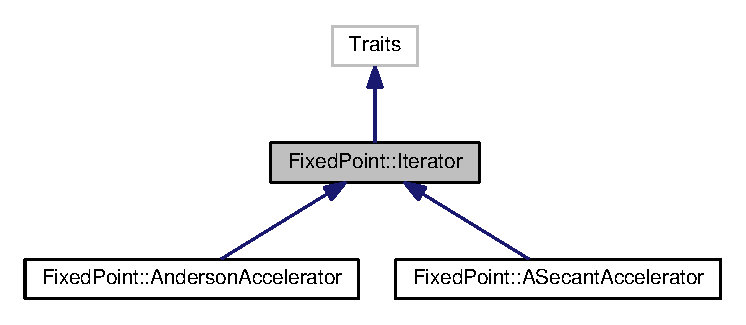
\includegraphics{./Include/inheritance.eps}
			\centering
			\caption{\textit{Inheritance diagram for the} \texttt{Iterator} \textit{class}}
			\label{fig:1}
		\end{figure}
		In addition to the \verb|AndersonAccelerator| class, another class called \verb|ASecantAccelerator| is provided,
		wihch implements a simpler version of Anderson algorithm in which the memory parameter has value two.
		
		Let us dive deeper into the implementation of Anderson algorithm.
		
		
		\subsection {Implementation of Anderson algorithm}
		Equation \ref{eq:2} shows that to compute the next value of the sequence two matrices are needed:
		$\mathscr{X}_k$ and $\mathscr{F}_k$.\\
		The \verb|AndersonAccelerator| class stores two matrices \verb|X| and \verb|F| which are updated 
		only in the last column at each call of the call operator.\\
		These two matrices have a special type to perform the update operation easily: it is the \verb|RotatingMatrix|
		template class. The template argument is chosen to provide the most efficient insert strategy, the one in which
		the new inserted column replaces the oldest column when the maximum size of the matrix has been reached.\\
		Since the call operator only updates the last column, it \textbf{can not} be called on a generic
		vector sequence but only on a sequence that was produced by the class itself.
		To circumvent this problem, the \verb|SetUp| method computes $\mathscr{X}_k$ and $\mathscr{F}_k$ up
		to the values involving the last iteration. If an Anderson step wants to be applied to a vector sequence
		produced in another way, the \verb|SetUp| method has to be called before the call operator.
		
		Concerning the update formula \ref{eq:2}, the term $\mathscr{F}_k^T \mathscr{F}_k^{-1}\mathscr{F}_k^T f_k$
		represents the solution of a least square problem. It is well known that solving this so-called normal
		equations is a bad choice from the numerical point of view, due to ill-conditioning of the matrices.
		For this reason, the least square problem is solved by mean of the QR decomposition of the matrix $\mathscr{F}_k$. In particular the
		Householder rank-revealing QR decomposition with column-pivoting is used, that is a good compromise
		between numerical stability and efficiency.\\
		Interestingly enough, the result of the update formula \ref{eq:2} is independent of the ordering of the columns
		of $\mathscr{X}_k$ and $\mathscr{F}_k$. This is relevant since 
		the proper reordering of the columns of the \verb|RotatingMatrix| class would add another computational cost.\\		
		The fact can be seen from the QR decomposition but is more easily seen from the normal equations.\\
		Calling $P$ a generic permutation matrix (which has the property
		that $P^T=P^{-1}$), swapping column of a matrix $A$ is achieved by performing the matrix multiplication $AP$.
		Substituting $\mathscr{X}_k$ and $\mathscr{F}_k$ with their permuted counterpart, eq. \ref{eq:2} becomes
		\begin{equation}
			x_{k+1}=x_{k} + \beta f_k -(\mathscr{X}_k + \beta \mathscr{F}_k)P(P^T \mathscr{F}_k^T \mathscr{F}_k P)^{-1}P^T \mathscr{F}_k^T f_k
		\end{equation}
		Thus, for properties of the inverse of a matrix
		\begin{equation}
			x_{k+1}=x_{k} + \beta f_k -(\mathscr{X}_k + \beta \mathscr{F}_k)P P^T (\mathscr{F}_k^T \mathscr{F}_k)^{-1} P P^T \mathscr{F}_k^T f_k
		\end{equation}
		By simplifying $P P^T$ we obtain that the solution is invariant with respect to permutation of columns of $\mathscr{X}_k$ and $\mathscr{F}_k$.
		
		One last note: \citeauthor{Walker} \cite{Walker} make use of factor-updating QR decomposition, which is a more efficient algorithm
		for computing the QR factors of $\mathscr{F}_k$ from the ones of $\mathscr{F}_{k-1}$. We did not consider it in this project
		because such algorithm was not available in the Eigen library. Moreover the rank-1 updated QR decomposition would not work
		when the oldest column of the matrix gets replaced.
		
		
		\subsection {The \texttt{FixedPointIterator} class}
		The \texttt{FixedPointIterator} class governs the solving of the fixed-point problem.\\
		It has the following private attributes:
		\begin{itemize}
		\item \verb|iterator|, an \verb|std::unique_ptr| to an \verb|Iterator| object that produces the iterates. The unique pointer
		allows to compose an object in the polymorphic \verb|Iterator| family, for example an \verb|AndersonAccelerator| object.
		\item \verb|options|, an options struct, controlling maximum iterations, tolerances and printing styles.
		\item \verb|history|, an \verb|std::deque<Vector>| containing the history of the vector sequence.\\
		\verb|std::deque| was prefered to \verb|std::vector| because when the number of stored vectors reaches the threshold
		of \verb|options::memory|, the oldest vector is eliminated from the front and the new vector is added to the back.
		This operation is much more efficient on \verb|std::deque|.
		\item \verb|iteration|, an integer representing the number of executed iterations by the \verb|compute| method.
		\end{itemize}
		
		Concerning the public member functions, the class  provides:
		\begin{itemize}
		\item a \verb|compute()| method taking no arguments
		\item a \verb|compute(const Vector&)| method taking an initial vector as a starting guess
		\item  methods to output a result (\verb|printResult| is one possibility).
		\end{itemize}
		The \verb|compute| methods make use of the \verb|history| member to compute iterations until
		convergence. In fact, the initial guess is used only in the case \verb|history| is empty. If \verb|history| is empty
		and no guess is provided, a default vector of zeros is used.\\
		
		\section{Examples and applications}
			\label{sec:app}
		
		\subsection{A first example}
			The file \verb|main_simple_problem.cpp| constitutes a first working example of the previously defined classes.\\
			It solves a simple nonlinear problem in 3D, taken from book \cite{Quarteroni}, whose fixed-point form converges to
			the solution $(0,1/3,0)$.\\
			All the parameters of interest are read from an input file, exploiting GetPot, a simple but effective utility.
			This allows to not recompile the code when we want to test a different parameter.
			
			\begin{figure}
			{\scriptsize
			% GNUPLOT: LaTeX picture with Postscript
\begingroup
  % Encoding inside the plot.  In the header of your document, this encoding
  % should to defined, e.g., by using
  % \usepackage[cp1252,<other encodings>]{inputenc}
  \inputencoding{cp1252}%
  \makeatletter
  \providecommand\color[2][]{%
    \GenericError{(gnuplot) \space\space\space\@spaces}{%
      Package color not loaded in conjunction with
      terminal option `colourtext'%
    }{See the gnuplot documentation for explanation.%
    }{Either use 'blacktext' in gnuplot or load the package
      color.sty in LaTeX.}%
    \renewcommand\color[2][]{}%
  }%
  \providecommand\includegraphics[2][]{%
    \GenericError{(gnuplot) \space\space\space\@spaces}{%
      Package graphicx or graphics not loaded%
    }{See the gnuplot documentation for explanation.%
    }{The gnuplot epslatex terminal needs graphicx.sty or graphics.sty.}%
    \renewcommand\includegraphics[2][]{}%
  }%
  \providecommand\rotatebox[2]{#2}%
  \@ifundefined{ifGPcolor}{%
    \newif\ifGPcolor
    \GPcolorfalse
  }{}%
  \@ifundefined{ifGPblacktext}{%
    \newif\ifGPblacktext
    \GPblacktexttrue
  }{}%
  % define a \g@addto@macro without @ in the name:
  \let\gplgaddtomacro\g@addto@macro
  % define empty templates for all commands taking text:
  \gdef\gplbacktext{}%
  \gdef\gplfronttext{}%
  \makeatother
  \ifGPblacktext
    % no textcolor at all
    \def\colorrgb#1{}%
    \def\colorgray#1{}%
  \else
    % gray or color?
    \ifGPcolor
      \def\colorrgb#1{\color[rgb]{#1}}%
      \def\colorgray#1{\color[gray]{#1}}%
      \expandafter\def\csname LTw\endcsname{\color{white}}%
      \expandafter\def\csname LTb\endcsname{\color{black}}%
      \expandafter\def\csname LTa\endcsname{\color{black}}%
      \expandafter\def\csname LT0\endcsname{\color[rgb]{1,0,0}}%
      \expandafter\def\csname LT1\endcsname{\color[rgb]{0,1,0}}%
      \expandafter\def\csname LT2\endcsname{\color[rgb]{0,0,1}}%
      \expandafter\def\csname LT3\endcsname{\color[rgb]{1,0,1}}%
      \expandafter\def\csname LT4\endcsname{\color[rgb]{0,1,1}}%
      \expandafter\def\csname LT5\endcsname{\color[rgb]{1,1,0}}%
      \expandafter\def\csname LT6\endcsname{\color[rgb]{0,0,0}}%
      \expandafter\def\csname LT7\endcsname{\color[rgb]{1,0.3,0}}%
      \expandafter\def\csname LT8\endcsname{\color[rgb]{0.5,0.5,0.5}}%
    \else
      % gray
      \def\colorrgb#1{\color{black}}%
      \def\colorgray#1{\color[gray]{#1}}%
      \expandafter\def\csname LTw\endcsname{\color{white}}%
      \expandafter\def\csname LTb\endcsname{\color{black}}%
      \expandafter\def\csname LTa\endcsname{\color{black}}%
      \expandafter\def\csname LT0\endcsname{\color{black}}%
      \expandafter\def\csname LT1\endcsname{\color{black}}%
      \expandafter\def\csname LT2\endcsname{\color{black}}%
      \expandafter\def\csname LT3\endcsname{\color{black}}%
      \expandafter\def\csname LT4\endcsname{\color{black}}%
      \expandafter\def\csname LT5\endcsname{\color{black}}%
      \expandafter\def\csname LT6\endcsname{\color{black}}%
      \expandafter\def\csname LT7\endcsname{\color{black}}%
      \expandafter\def\csname LT8\endcsname{\color{black}}%
    \fi
  \fi
    \setlength{\unitlength}{0.0500bp}%
    \ifx\gptboxheight\undefined%
      \newlength{\gptboxheight}%
      \newlength{\gptboxwidth}%
      \newsavebox{\gptboxtext}%
    \fi%
    \setlength{\fboxrule}{0.5pt}%
    \setlength{\fboxsep}{1pt}%
\begin{picture}(5668.00,2834.00)%
    \gplgaddtomacro\gplbacktext{%
      \csname LTb\endcsname%%
      \put(1220,806){\makebox(0,0)[r]{\strut{}$1\times10^{-10}$}}%
      \put(1220,1138){\makebox(0,0)[r]{\strut{}$1\times10^{-8}$}}%
      \put(1220,1470){\makebox(0,0)[r]{\strut{}$1\times10^{-6}$}}%
      \put(1220,1803){\makebox(0,0)[r]{\strut{}$0.0001$}}%
      \put(1220,2135){\makebox(0,0)[r]{\strut{}$0.01$}}%
      \put(1220,2467){\makebox(0,0)[r]{\strut{}$1$}}%
      \put(1340,440){\makebox(0,0){\strut{}$0$}}%
      \put(2001,440){\makebox(0,0){\strut{}$5$}}%
      \put(2662,440){\makebox(0,0){\strut{}$10$}}%
      \put(3324,440){\makebox(0,0){\strut{}$15$}}%
      \put(3985,440){\makebox(0,0){\strut{}$20$}}%
      \put(4646,440){\makebox(0,0){\strut{}$25$}}%
      \put(5307,440){\makebox(0,0){\strut{}$30$}}%
    }%
    \gplgaddtomacro\gplfronttext{%
      \csname LTb\endcsname%%
      \put(190,1636){\rotatebox{-270}{\makebox(0,0){\strut{}Residual}}}%
      \put(3323,140){\makebox(0,0){\strut{}Iteration \#}}%
      \csname LTb\endcsname%%
      \put(4404,2470){\makebox(0,0)[r]{\strut{}Fixed-point iterations}}%
      \csname LTb\endcsname%%
      \put(4404,2270){\makebox(0,0)[r]{\strut{}Anderson algorithm}}%
    }%
    \gplbacktext
    \put(0,0){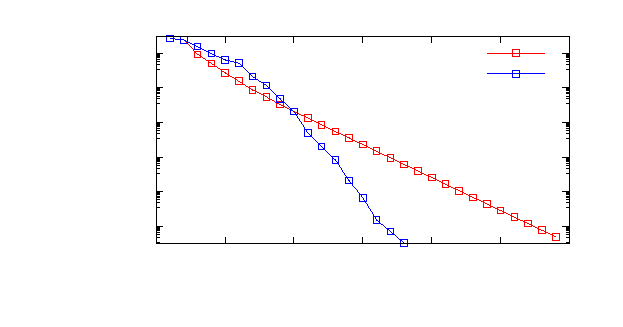
\includegraphics{./Include/simple_example_residuals}}%
    \gplfronttext
  \end{picture}%
\endgroup
}
			\centering
			\caption{\textit{Residual vs Interation number for the nonlinear 3D problem}}
			\label{fig:simple}
			\end{figure}
			
			Figure \ref{fig:simple} shows the residual at each iteration when standard fixed-point iterations are used 
			and when Anderson algorithm is used. Parameters of Anderson algorithm are $\beta=1$ and memory $m=5$.\\
			Fixed-point iterations converge in $28$ iterations whereas Anderson algorithm converges in $17$.
			
		\subsection{A linear FEM example}
			The file \verb|main_gauss_seidel.cpp| solves the heat equation, in the form of a diffusion
			reaction problem, on a one-dimensional bar with Dirichlet condition on one side and Neumann condition on the other.
			For further description, consult \cite{Formaggia}.\\
			By FEM discretization (or equivalently by finite differences, since we are in 1D), a tridiagonal matrix is obtained.\\
			We decided to implement the simple Gauss-Seidel iterative scheme, notoriously slow.
			\begin{figure}
			{\scriptsize
			% GNUPLOT: LaTeX picture with Postscript
\begingroup
  % Encoding inside the plot.  In the header of your document, this encoding
  % should to defined, e.g., by using
  % \usepackage[cp1252,<other encodings>]{inputenc}
  \inputencoding{cp1252}%
  \makeatletter
  \providecommand\color[2][]{%
    \GenericError{(gnuplot) \space\space\space\@spaces}{%
      Package color not loaded in conjunction with
      terminal option `colourtext'%
    }{See the gnuplot documentation for explanation.%
    }{Either use 'blacktext' in gnuplot or load the package
      color.sty in LaTeX.}%
    \renewcommand\color[2][]{}%
  }%
  \providecommand\includegraphics[2][]{%
    \GenericError{(gnuplot) \space\space\space\@spaces}{%
      Package graphicx or graphics not loaded%
    }{See the gnuplot documentation for explanation.%
    }{The gnuplot epslatex terminal needs graphicx.sty or graphics.sty.}%
    \renewcommand\includegraphics[2][]{}%
  }%
  \providecommand\rotatebox[2]{#2}%
  \@ifundefined{ifGPcolor}{%
    \newif\ifGPcolor
    \GPcolorfalse
  }{}%
  \@ifundefined{ifGPblacktext}{%
    \newif\ifGPblacktext
    \GPblacktexttrue
  }{}%
  % define a \g@addto@macro without @ in the name:
  \let\gplgaddtomacro\g@addto@macro
  % define empty templates for all commands taking text:
  \gdef\gplbacktext{}%
  \gdef\gplfronttext{}%
  \makeatother
  \ifGPblacktext
    % no textcolor at all
    \def\colorrgb#1{}%
    \def\colorgray#1{}%
  \else
    % gray or color?
    \ifGPcolor
      \def\colorrgb#1{\color[rgb]{#1}}%
      \def\colorgray#1{\color[gray]{#1}}%
      \expandafter\def\csname LTw\endcsname{\color{white}}%
      \expandafter\def\csname LTb\endcsname{\color{black}}%
      \expandafter\def\csname LTa\endcsname{\color{black}}%
      \expandafter\def\csname LT0\endcsname{\color[rgb]{1,0,0}}%
      \expandafter\def\csname LT1\endcsname{\color[rgb]{0,1,0}}%
      \expandafter\def\csname LT2\endcsname{\color[rgb]{0,0,1}}%
      \expandafter\def\csname LT3\endcsname{\color[rgb]{1,0,1}}%
      \expandafter\def\csname LT4\endcsname{\color[rgb]{0,1,1}}%
      \expandafter\def\csname LT5\endcsname{\color[rgb]{1,1,0}}%
      \expandafter\def\csname LT6\endcsname{\color[rgb]{0,0,0}}%
      \expandafter\def\csname LT7\endcsname{\color[rgb]{1,0.3,0}}%
      \expandafter\def\csname LT8\endcsname{\color[rgb]{0.5,0.5,0.5}}%
    \else
      % gray
      \def\colorrgb#1{\color{black}}%
      \def\colorgray#1{\color[gray]{#1}}%
      \expandafter\def\csname LTw\endcsname{\color{white}}%
      \expandafter\def\csname LTb\endcsname{\color{black}}%
      \expandafter\def\csname LTa\endcsname{\color{black}}%
      \expandafter\def\csname LT0\endcsname{\color{black}}%
      \expandafter\def\csname LT1\endcsname{\color{black}}%
      \expandafter\def\csname LT2\endcsname{\color{black}}%
      \expandafter\def\csname LT3\endcsname{\color{black}}%
      \expandafter\def\csname LT4\endcsname{\color{black}}%
      \expandafter\def\csname LT5\endcsname{\color{black}}%
      \expandafter\def\csname LT6\endcsname{\color{black}}%
      \expandafter\def\csname LT7\endcsname{\color{black}}%
      \expandafter\def\csname LT8\endcsname{\color{black}}%
    \fi
  \fi
    \setlength{\unitlength}{0.0500bp}%
    \ifx\gptboxheight\undefined%
      \newlength{\gptboxheight}%
      \newlength{\gptboxwidth}%
      \newsavebox{\gptboxtext}%
    \fi%
    \setlength{\fboxrule}{0.5pt}%
    \setlength{\fboxsep}{1pt}%
\begin{picture}(5668.00,2834.00)%
    \gplgaddtomacro\gplbacktext{%
      \csname LTb\endcsname%%
      \put(1342,704){\makebox(0,0)[r]{\strut{}$1\times10^{-12}$}}%
      \put(1342,1051){\makebox(0,0)[r]{\strut{}$1\times10^{-10}$}}%
      \put(1342,1398){\makebox(0,0)[r]{\strut{}$1\times10^{-8}$}}%
      \put(1342,1745){\makebox(0,0)[r]{\strut{}$1\times10^{-6}$}}%
      \put(1342,2092){\makebox(0,0)[r]{\strut{}$0.0001$}}%
      \put(1342,2439){\makebox(0,0)[r]{\strut{}$0.01$}}%
      \put(1474,484){\makebox(0,0){\strut{}$0$}}%
      \put(1949,484){\makebox(0,0){\strut{}$10$}}%
      \put(2423,484){\makebox(0,0){\strut{}$20$}}%
      \put(2898,484){\makebox(0,0){\strut{}$30$}}%
      \put(3373,484){\makebox(0,0){\strut{}$40$}}%
      \put(3847,484){\makebox(0,0){\strut{}$50$}}%
      \put(4322,484){\makebox(0,0){\strut{}$60$}}%
      \put(4796,484){\makebox(0,0){\strut{}$70$}}%
      \put(5271,484){\makebox(0,0){\strut{}$80$}}%
    }%
    \gplgaddtomacro\gplfronttext{%
      \csname LTb\endcsname%%
      \put(209,1658){\rotatebox{-270}{\makebox(0,0){\strut{}Residual}}}%
      \put(3372,154){\makebox(0,0){\strut{}Iteration \#}}%
      \csname LTb\endcsname%%
      \put(2461,1097){\makebox(0,0)[l]{\strut{}Gauss-Seidel iterations}}%
      \csname LTb\endcsname%%
      \put(2461,877){\makebox(0,0)[l]{\strut{}Anderson algorithm}}%
    }%
    \gplbacktext
    \put(0,0){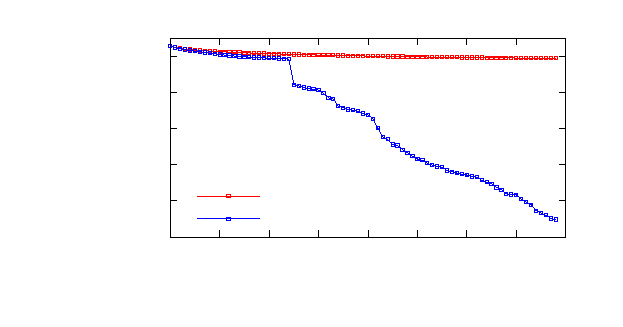
\includegraphics{gauss}}%
    \gplfronttext
  \end{picture}%
\endgroup
}
			\centering
			\caption{\textit{Residual vs Interation number for the Gauss-Seidel problem}}
			\label{fig:Gauss}
			\end{figure}
			Using as parameters of Anderson algorithm the same as the example before, and as mesh size $25$, we can observe in fig.\ref{fig:Gauss} that Anderson
			accelerator does a good job at accelerating this method: the Gauss-Seidel method would need $3339$ iterations
			to converge!
			
			An analysis concerning the parameters $m$ and $\beta$ was carried out for this example. In fig. \ref{fig:Heat}
			\begin{figure}
			{\scriptsize
			% GNUPLOT: LaTeX picture with Postscript
\begingroup
  % Encoding inside the plot.  In the header of your document, this encoding
  % should to defined, e.g., by using
  % \usepackage[cp1252,<other encodings>]{inputenc}
  \inputencoding{cp1252}%
  \makeatletter
  \providecommand\color[2][]{%
    \GenericError{(gnuplot) \space\space\space\@spaces}{%
      Package color not loaded in conjunction with
      terminal option `colourtext'%
    }{See the gnuplot documentation for explanation.%
    }{Either use 'blacktext' in gnuplot or load the package
      color.sty in LaTeX.}%
    \renewcommand\color[2][]{}%
  }%
  \providecommand\includegraphics[2][]{%
    \GenericError{(gnuplot) \space\space\space\@spaces}{%
      Package graphicx or graphics not loaded%
    }{See the gnuplot documentation for explanation.%
    }{The gnuplot epslatex terminal needs graphicx.sty or graphics.sty.}%
    \renewcommand\includegraphics[2][]{}%
  }%
  \providecommand\rotatebox[2]{#2}%
  \@ifundefined{ifGPcolor}{%
    \newif\ifGPcolor
    \GPcolortrue
  }{}%
  \@ifundefined{ifGPblacktext}{%
    \newif\ifGPblacktext
    \GPblacktexttrue
  }{}%
  % define a \g@addto@macro without @ in the name:
  \let\gplgaddtomacro\g@addto@macro
  % define empty templates for all commands taking text:
  \gdef\gplbacktext{}%
  \gdef\gplfronttext{}%
  \makeatother
  \ifGPblacktext
    % no textcolor at all
    \def\colorrgb#1{}%
    \def\colorgray#1{}%
  \else
    % gray or color?
    \ifGPcolor
      \def\colorrgb#1{\color[rgb]{#1}}%
      \def\colorgray#1{\color[gray]{#1}}%
      \expandafter\def\csname LTw\endcsname{\color{white}}%
      \expandafter\def\csname LTb\endcsname{\color{black}}%
      \expandafter\def\csname LTa\endcsname{\color{black}}%
      \expandafter\def\csname LT0\endcsname{\color[rgb]{1,0,0}}%
      \expandafter\def\csname LT1\endcsname{\color[rgb]{0,1,0}}%
      \expandafter\def\csname LT2\endcsname{\color[rgb]{0,0,1}}%
      \expandafter\def\csname LT3\endcsname{\color[rgb]{1,0,1}}%
      \expandafter\def\csname LT4\endcsname{\color[rgb]{0,1,1}}%
      \expandafter\def\csname LT5\endcsname{\color[rgb]{1,1,0}}%
      \expandafter\def\csname LT6\endcsname{\color[rgb]{0,0,0}}%
      \expandafter\def\csname LT7\endcsname{\color[rgb]{1,0.3,0}}%
      \expandafter\def\csname LT8\endcsname{\color[rgb]{0.5,0.5,0.5}}%
    \else
      % gray
      \def\colorrgb#1{\color{black}}%
      \def\colorgray#1{\color[gray]{#1}}%
      \expandafter\def\csname LTw\endcsname{\color{white}}%
      \expandafter\def\csname LTb\endcsname{\color{black}}%
      \expandafter\def\csname LTa\endcsname{\color{black}}%
      \expandafter\def\csname LT0\endcsname{\color{black}}%
      \expandafter\def\csname LT1\endcsname{\color{black}}%
      \expandafter\def\csname LT2\endcsname{\color{black}}%
      \expandafter\def\csname LT3\endcsname{\color{black}}%
      \expandafter\def\csname LT4\endcsname{\color{black}}%
      \expandafter\def\csname LT5\endcsname{\color{black}}%
      \expandafter\def\csname LT6\endcsname{\color{black}}%
      \expandafter\def\csname LT7\endcsname{\color{black}}%
      \expandafter\def\csname LT8\endcsname{\color{black}}%
    \fi
  \fi
    \setlength{\unitlength}{0.0500bp}%
    \ifx\gptboxheight\undefined%
      \newlength{\gptboxheight}%
      \newlength{\gptboxwidth}%
      \newsavebox{\gptboxtext}%
    \fi%
    \setlength{\fboxrule}{0.5pt}%
    \setlength{\fboxsep}{1pt}%
\begin{picture}(9070.00,4534.00)%
    \gplgaddtomacro\gplbacktext{%
      \csname LTb\endcsname%%
      \put(682,930){\makebox(0,0)[r]{\strut{}2}}%
      \put(682,1381){\makebox(0,0)[r]{\strut{}4}}%
      \put(682,1832){\makebox(0,0)[r]{\strut{}6}}%
      \put(682,2283){\makebox(0,0)[r]{\strut{}8}}%
      \put(682,2734){\makebox(0,0)[r]{\strut{}10}}%
      \put(682,3185){\makebox(0,0)[r]{\strut{}15}}%
      \put(682,3636){\makebox(0,0)[r]{\strut{}20}}%
      \put(682,4087){\makebox(0,0)[r]{\strut{}25}}%
      \put(1052,484){\makebox(0,0){\strut{}1e-06}}%
      \put(1528,484){\makebox(0,0){\strut{}1e-05}}%
      \put(2004,484){\makebox(0,0){\strut{}0.0001}}%
      \put(2480,484){\makebox(0,0){\strut{}0.001}}%
      \put(2956,484){\makebox(0,0){\strut{}0.01}}%
      \put(3432,484){\makebox(0,0){\strut{}0.1}}%
      \put(3908,484){\makebox(0,0){\strut{}0.5}}%
      \put(4383,484){\makebox(0,0){\strut{}1}}%
      \put(4859,484){\makebox(0,0){\strut{}2}}%
      \put(5335,484){\makebox(0,0){\strut{}5}}%
      \put(5811,484){\makebox(0,0){\strut{}10}}%
      \put(6287,484){\makebox(0,0){\strut{}50}}%
      \put(6763,484){\makebox(0,0){\strut{}100}}%
      \put(7239,484){\makebox(0,0){\strut{}1000}}%
    }%
    \gplgaddtomacro\gplfronttext{%
      \csname LTb\endcsname%%
      \put(209,2508){\rotatebox{-270}{\makebox(0,0){\strut{}$m$ (memory)}}}%
      \put(4145,154){\makebox(0,0){\strut{}$\beta$ (relaxation)}}%
      \csname LTb\endcsname%%
      \put(8109,1190){\makebox(0,0)[l]{\strut{}$0.001$}}%
      \put(8109,2657){\makebox(0,0)[l]{\strut{}$0.01$}}%
      \put(8109,4125){\makebox(0,0)[l]{\strut{}$0.1$}}%
      \put(8835,2508){\rotatebox{-270}{\makebox(0,0){\strut{}Time taken ($s$)}}}%
    }%
    \gplbacktext
    \put(0,0){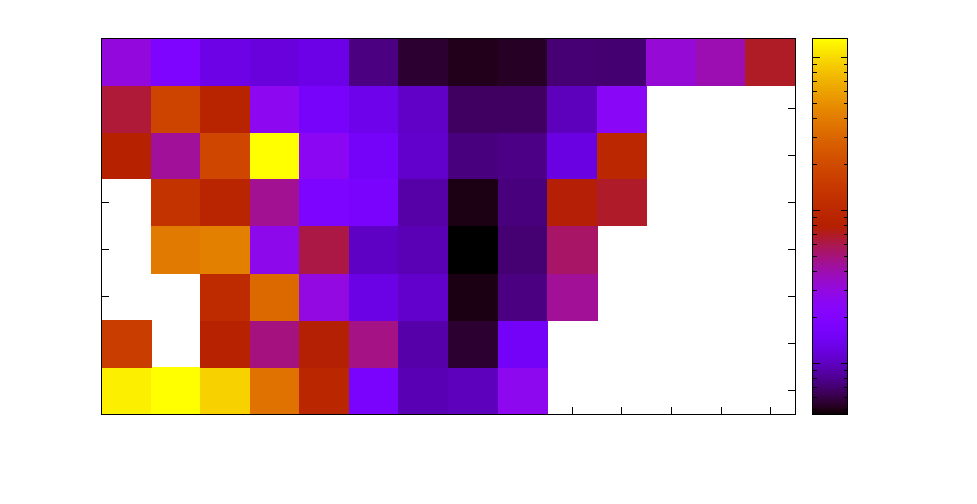
\includegraphics{heat_map}}%
    \gplfronttext
  \end{picture}%
\endgroup
}
			\centering
			\caption{\textit{Heat map of execution time with different values of the parameters $m$ and $\beta$: the darker means the code was faster. White squares means
			convergence was not reached.}}
			\label{fig:Heat}
			\end{figure}
			the heat map represents on a log-scale the time needed to reach convergence.
			Where the map is white, it means the iterations did not converge (they most likely
			diverged). For every parameter set the code was executed $10$ times to obtain an average execution time.\\
			You can see that $\beta=1$ is by far the best choice, while for the memory parameter
			several choices are good. For high number of the memory parameter, the code converged in less than
			$30$	iterations, so increasing $m$ would not change the result.
			
			Also a simple profiling of the code has been performed, through \verb|gprof|. It showed
			that most of the execution time for the Anderson iterations, by far, is spent
			in the QR decomposition of the $\mathscr{F}_k$ matrix (run
			\verb|make profiler| for seeing with your eyes in the generated \verb|profiling.txt| file).
			
		\subsection{Alternating method}
			Following the idea in paper \cite{Pratapa}, an alternating Anderson scheme was implemented.\\
			The idea is to run simple fixed-point interations for a number $p$ of iterations, followed by
			an Anderson step and keep alternating in such a way. It is particularly good when applied
			to the Jacobi iterative scheme because it can be simply implemented
			in a parallel architecture.\\
			Since I am using a normal computer, I have used instead the Gauss-Seidel scheme of the previous example,
			but changing two characters in the code would transform the Gauss-Seidel method into the Jacobi method,
			without substantially changing the results.
			
			Implementation-wise, I chose to exploit all the functionalities provided by the interface
			to implement the alternating scheme in	\verb|main_gauss_seidel.cpp|, rather than
			wrapping \verb|AndersonAccelerator| into a suitable \verb|Iterator| class. 
			The \verb|swap| method of \verb|std::unique_ptr| was used for alternating the \verb|AndersonAccelerator|
			and the \verb|Iterator| classes stored in the \verb|FixedPointIterator| object.
			
			Different values of the number $p$ have been tested for parameters $\beta=1$ and memory $m=8$, but very similar behaviour
			is observed for different values of $m$. Fig. \ref{fig:tab1} shows that increasing $p$ to a value slightly greater than
			$m$ accelerates the process. It is not shown in the figure, but note that the standard Anderson method converges in
			about $0.0005 s$.\\
			With the alternating method we were able to reach a speed-up of almost 10, which is quite impressive.
			
			% \begin{table}
			% \resizebox{\textwidth}{!}{
			% \begin{tabular}
			% { |c|c|c|c|c|c|c|c|c|c|c|c|c|c|c|c|c|c|c|c| }
			% \hline
			% $p$ & 0 & 2	& 4 & 6 & 8 & 10 & 12 & 14 & 16 & 18\\
			% \hline
			% time ($10^{-4}s$) & 5.07 & 2.31 & 1.67 & 1.88 & 2.76 & 1.69 & 2.19 & 1.27 & 1.28 & 0.99\\
			% \hline
			% \end{tabular}}
			% \end{table}
			
			\begin{figure}
			{\scriptsize
			% GNUPLOT: LaTeX picture with Postscript
\begingroup
  % Encoding inside the plot.  In the header of your document, this encoding
  % should to defined, e.g., by using
  % \usepackage[cp1252,<other encodings>]{inputenc}
  \inputencoding{cp1252}%
  \makeatletter
  \providecommand\color[2][]{%
    \GenericError{(gnuplot) \space\space\space\@spaces}{%
      Package color not loaded in conjunction with
      terminal option `colourtext'%
    }{See the gnuplot documentation for explanation.%
    }{Either use 'blacktext' in gnuplot or load the package
      color.sty in LaTeX.}%
    \renewcommand\color[2][]{}%
  }%
  \providecommand\includegraphics[2][]{%
    \GenericError{(gnuplot) \space\space\space\@spaces}{%
      Package graphicx or graphics not loaded%
    }{See the gnuplot documentation for explanation.%
    }{The gnuplot epslatex terminal needs graphicx.sty or graphics.sty.}%
    \renewcommand\includegraphics[2][]{}%
  }%
  \providecommand\rotatebox[2]{#2}%
  \@ifundefined{ifGPcolor}{%
    \newif\ifGPcolor
    \GPcolorfalse
  }{}%
  \@ifundefined{ifGPblacktext}{%
    \newif\ifGPblacktext
    \GPblacktexttrue
  }{}%
  % define a \g@addto@macro without @ in the name:
  \let\gplgaddtomacro\g@addto@macro
  % define empty templates for all commands taking text:
  \gdef\gplbacktext{}%
  \gdef\gplfronttext{}%
  \makeatother
  \ifGPblacktext
    % no textcolor at all
    \def\colorrgb#1{}%
    \def\colorgray#1{}%
  \else
    % gray or color?
    \ifGPcolor
      \def\colorrgb#1{\color[rgb]{#1}}%
      \def\colorgray#1{\color[gray]{#1}}%
      \expandafter\def\csname LTw\endcsname{\color{white}}%
      \expandafter\def\csname LTb\endcsname{\color{black}}%
      \expandafter\def\csname LTa\endcsname{\color{black}}%
      \expandafter\def\csname LT0\endcsname{\color[rgb]{1,0,0}}%
      \expandafter\def\csname LT1\endcsname{\color[rgb]{0,1,0}}%
      \expandafter\def\csname LT2\endcsname{\color[rgb]{0,0,1}}%
      \expandafter\def\csname LT3\endcsname{\color[rgb]{1,0,1}}%
      \expandafter\def\csname LT4\endcsname{\color[rgb]{0,1,1}}%
      \expandafter\def\csname LT5\endcsname{\color[rgb]{1,1,0}}%
      \expandafter\def\csname LT6\endcsname{\color[rgb]{0,0,0}}%
      \expandafter\def\csname LT7\endcsname{\color[rgb]{1,0.3,0}}%
      \expandafter\def\csname LT8\endcsname{\color[rgb]{0.5,0.5,0.5}}%
    \else
      % gray
      \def\colorrgb#1{\color{black}}%
      \def\colorgray#1{\color[gray]{#1}}%
      \expandafter\def\csname LTw\endcsname{\color{white}}%
      \expandafter\def\csname LTb\endcsname{\color{black}}%
      \expandafter\def\csname LTa\endcsname{\color{black}}%
      \expandafter\def\csname LT0\endcsname{\color{black}}%
      \expandafter\def\csname LT1\endcsname{\color{black}}%
      \expandafter\def\csname LT2\endcsname{\color{black}}%
      \expandafter\def\csname LT3\endcsname{\color{black}}%
      \expandafter\def\csname LT4\endcsname{\color{black}}%
      \expandafter\def\csname LT5\endcsname{\color{black}}%
      \expandafter\def\csname LT6\endcsname{\color{black}}%
      \expandafter\def\csname LT7\endcsname{\color{black}}%
      \expandafter\def\csname LT8\endcsname{\color{black}}%
    \fi
  \fi
    \setlength{\unitlength}{0.0500bp}%
    \ifx\gptboxheight\undefined%
      \newlength{\gptboxheight}%
      \newlength{\gptboxwidth}%
      \newsavebox{\gptboxtext}%
    \fi%
    \setlength{\fboxrule}{0.5pt}%
    \setlength{\fboxsep}{1pt}%
\begin{picture}(5668.00,2834.00)%
    \gplgaddtomacro\gplbacktext{%
      \csname LTb\endcsname%%
      \put(1342,704){\makebox(0,0)[r]{\strut{}0.00005}}%
      \put(1342,1086){\makebox(0,0)[r]{\strut{}0.00010}}%
      \put(1342,1468){\makebox(0,0)[r]{\strut{}0.00015}}%
      \put(1342,1849){\makebox(0,0)[r]{\strut{}0.00020}}%
      \put(1342,2231){\makebox(0,0)[r]{\strut{}0.00025}}%
      \put(1342,2613){\makebox(0,0)[r]{\strut{}0.00030}}%
      \put(1474,484){\makebox(0,0){\strut{}$0$}}%
      \put(1854,484){\makebox(0,0){\strut{}$20$}}%
      \put(2233,484){\makebox(0,0){\strut{}$40$}}%
      \put(2613,484){\makebox(0,0){\strut{}$60$}}%
      \put(2993,484){\makebox(0,0){\strut{}$80$}}%
      \put(3373,484){\makebox(0,0){\strut{}$100$}}%
      \put(3752,484){\makebox(0,0){\strut{}$120$}}%
      \put(4132,484){\makebox(0,0){\strut{}$140$}}%
      \put(4512,484){\makebox(0,0){\strut{}$160$}}%
      \put(4891,484){\makebox(0,0){\strut{}$180$}}%
      \put(5271,484){\makebox(0,0){\strut{}$200$}}%
    }%
    \gplgaddtomacro\gplfronttext{%
      \csname LTb\endcsname%%
      \put(209,1658){\rotatebox{-270}{\makebox(0,0){\strut{}time($s$)}}}%
      \put(3372,154){\makebox(0,0){\strut{}$p$}}%
    }%
    \gplbacktext
    \put(0,0){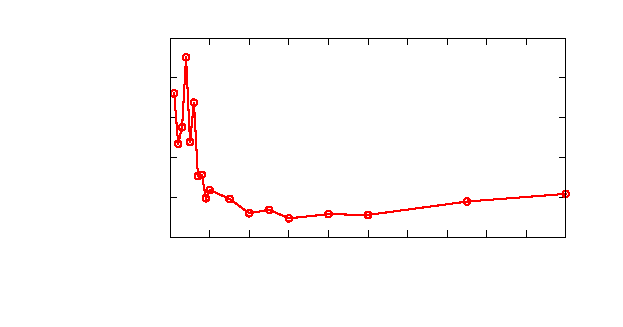
\includegraphics{alternating}}%
    \gplfronttext
  \end{picture}%
\endgroup
}
			\centering
			\caption{\textit{Testing different values of parameter $p$ with $\beta=1$ and $m=8$}}
			\label{fig:tab1}
			\end{figure}
			
			
			
			\subsection{Nonlinear FEM example}
			To study a nonlinear problem, we decided to add to the heat equation of previous examples a thermal radiation term.\\
			At the discrete level, this means solving the nonlinear system of equations
			\begin{equation}
				\label{eq:non}
				A u + \sigma I u^4 = f
			\end{equation}
			where $A$ is the same finite elements matrix corresponding to the previous example, whose exact form is found in
			\cite{Formaggia}, $I$ is the identity matrix, $\sigma$ is the radiation coefficient and $f$ is an
			appropriate right-hand side (I did not stick to the physics of the problem, because the radiation term
			is usually negligible, so I assigned $\sigma=1$ and I did not account for necessary corrections of the right-hand
			side).
			
			This formulation is easy to derive when we approximate the problem with finite differences, while
			with the use of finite elements it is obtained through the lumping of the mass matrix, a procedure
			used to avoid extra-diagonal terms.
			
			We solve system \ref{eq:non} written in a fixed-point form in the following manner:
			\begin{equation}
				u = (A+ \sigma I u^3)^{-1} f 
			\end{equation}
			resulting in the iterative scheme
			\begin{equation}
				\label{eq:nonfix}
				u_{k+1}= (A+ \sigma I u^3_k)^{-1} f 
			\end{equation}
			This in turns results in solving at each step the linear system
			\begin{equation}
				(A+ \sigma I u^3_k) u_{k+1} = f
			\end{equation}
			which is always possible being the corresponding matrix positive definite.\\
			This step was performed in the same manner of previous section, that is through the
			\verb|FixedPointIterator| class, accelerating the Gauss-Seidel iterative procedure
			with the alternating Anderson scheme.
			We have therefore created a fixed-point problem inside another fixed-point problem.\\
			In case the inner iterator does not converge, the code exits throwing a run-time
			exception (but given a suitable number of iterations it should always converge
			thanks to the properties of the Gauss-Seidel scheme).
			
			In fig. \ref{fig:nonlinear} you can see the residual history for the iterative scheme \ref{eq:nonfix}
			for different solvers.
			\begin{figure}
				{\scriptsize
			% GNUPLOT: LaTeX picture with Postscript
\begingroup
  % Encoding inside the plot.  In the header of your document, this encoding
  % should to defined, e.g., by using
  % \usepackage[cp1252,<other encodings>]{inputenc}
  \inputencoding{cp1252}%
  \makeatletter
  \providecommand\color[2][]{%
    \GenericError{(gnuplot) \space\space\space\@spaces}{%
      Package color not loaded in conjunction with
      terminal option `colourtext'%
    }{See the gnuplot documentation for explanation.%
    }{Either use 'blacktext' in gnuplot or load the package
      color.sty in LaTeX.}%
    \renewcommand\color[2][]{}%
  }%
  \providecommand\includegraphics[2][]{%
    \GenericError{(gnuplot) \space\space\space\@spaces}{%
      Package graphicx or graphics not loaded%
    }{See the gnuplot documentation for explanation.%
    }{The gnuplot epslatex terminal needs graphicx.sty or graphics.sty.}%
    \renewcommand\includegraphics[2][]{}%
  }%
  \providecommand\rotatebox[2]{#2}%
  \@ifundefined{ifGPcolor}{%
    \newif\ifGPcolor
    \GPcolorfalse
  }{}%
  \@ifundefined{ifGPblacktext}{%
    \newif\ifGPblacktext
    \GPblacktexttrue
  }{}%
  % define a \g@addto@macro without @ in the name:
  \let\gplgaddtomacro\g@addto@macro
  % define empty templates for all commands taking text:
  \gdef\gplbacktext{}%
  \gdef\gplfronttext{}%
  \makeatother
  \ifGPblacktext
    % no textcolor at all
    \def\colorrgb#1{}%
    \def\colorgray#1{}%
  \else
    % gray or color?
    \ifGPcolor
      \def\colorrgb#1{\color[rgb]{#1}}%
      \def\colorgray#1{\color[gray]{#1}}%
      \expandafter\def\csname LTw\endcsname{\color{white}}%
      \expandafter\def\csname LTb\endcsname{\color{black}}%
      \expandafter\def\csname LTa\endcsname{\color{black}}%
      \expandafter\def\csname LT0\endcsname{\color[rgb]{1,0,0}}%
      \expandafter\def\csname LT1\endcsname{\color[rgb]{0,1,0}}%
      \expandafter\def\csname LT2\endcsname{\color[rgb]{0,0,1}}%
      \expandafter\def\csname LT3\endcsname{\color[rgb]{1,0,1}}%
      \expandafter\def\csname LT4\endcsname{\color[rgb]{0,1,1}}%
      \expandafter\def\csname LT5\endcsname{\color[rgb]{1,1,0}}%
      \expandafter\def\csname LT6\endcsname{\color[rgb]{0,0,0}}%
      \expandafter\def\csname LT7\endcsname{\color[rgb]{1,0.3,0}}%
      \expandafter\def\csname LT8\endcsname{\color[rgb]{0.5,0.5,0.5}}%
    \else
      % gray
      \def\colorrgb#1{\color{black}}%
      \def\colorgray#1{\color[gray]{#1}}%
      \expandafter\def\csname LTw\endcsname{\color{white}}%
      \expandafter\def\csname LTb\endcsname{\color{black}}%
      \expandafter\def\csname LTa\endcsname{\color{black}}%
      \expandafter\def\csname LT0\endcsname{\color{black}}%
      \expandafter\def\csname LT1\endcsname{\color{black}}%
      \expandafter\def\csname LT2\endcsname{\color{black}}%
      \expandafter\def\csname LT3\endcsname{\color{black}}%
      \expandafter\def\csname LT4\endcsname{\color{black}}%
      \expandafter\def\csname LT5\endcsname{\color{black}}%
      \expandafter\def\csname LT6\endcsname{\color{black}}%
      \expandafter\def\csname LT7\endcsname{\color{black}}%
      \expandafter\def\csname LT8\endcsname{\color{black}}%
    \fi
  \fi
    \setlength{\unitlength}{0.0500bp}%
    \ifx\gptboxheight\undefined%
      \newlength{\gptboxheight}%
      \newlength{\gptboxwidth}%
      \newsavebox{\gptboxtext}%
    \fi%
    \setlength{\fboxrule}{0.5pt}%
    \setlength{\fboxsep}{1pt}%
\begin{picture}(5668.00,2834.00)%
    \gplgaddtomacro\gplbacktext{%
      \csname LTb\endcsname%%
      \put(1210,895){\makebox(0,0)[r]{\strut{}$1\times10^{-8}$}}%
      \put(1210,1277){\makebox(0,0)[r]{\strut{}$1\times10^{-6}$}}%
      \put(1210,1659){\makebox(0,0)[r]{\strut{}$0.0001$}}%
      \put(1210,2040){\makebox(0,0)[r]{\strut{}$0.01$}}%
      \put(1210,2422){\makebox(0,0)[r]{\strut{}$1$}}%
      \put(1342,484){\makebox(0,0){\strut{}$0$}}%
      \put(2128,484){\makebox(0,0){\strut{}$5$}}%
      \put(2914,484){\makebox(0,0){\strut{}$10$}}%
      \put(3699,484){\makebox(0,0){\strut{}$15$}}%
      \put(4485,484){\makebox(0,0){\strut{}$20$}}%
      \put(5271,484){\makebox(0,0){\strut{}$25$}}%
    }%
    \gplgaddtomacro\gplfronttext{%
      \csname LTb\endcsname%%
      \put(209,1658){\rotatebox{-270}{\makebox(0,0){\strut{}Residual}}}%
      \put(3306,154){\makebox(0,0){\strut{}Iteration \#}}%
      \csname LTb\endcsname%%
      \put(4284,2440){\makebox(0,0)[r]{\strut{}Fixed-point iterations}}%
      \csname LTb\endcsname%%
      \put(4284,2220){\makebox(0,0)[r]{\strut{}Newton iterations}}%
      \csname LTb\endcsname%%
      \put(4284,2000){\makebox(0,0)[r]{\strut{}Anderson iterations}}%
      \csname LTb\endcsname%%
      \put(4284,1780){\makebox(0,0)[r]{\strut{}Newton-Anderson}}%
    }%
    \gplbacktext
    \put(0,0){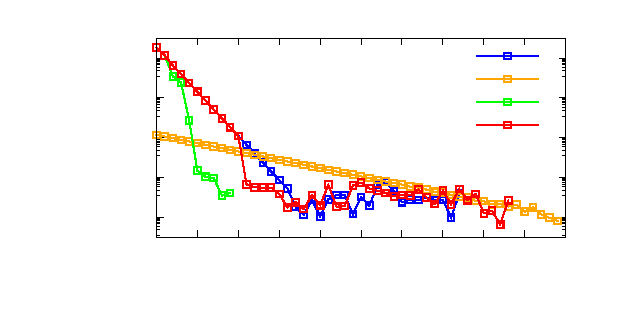
\includegraphics{nonlinear}}%
    \gplfronttext
  \end{picture}%
\endgroup
}
			\centering
			\caption{\textit{Residual vs Interation number for the nonlinear problem}}
			\label{fig:nonlinear}
			\end{figure}
			The fixed-point solver has linear convergence, as it usually happens.
			Anderson accelerator manages to speed-up significantly the fixed-point iterations and is able
			to converge in very few iterations. Alternating Anderson seems not to benefit particularly of
			the normal fixed-point iterations and much more from the Anderson step, but this can not be said
			from just this figure.\\
			The Newton method for problem \ref{eq:non} reads
			\begin{equation}
				x_{k+1}= x_k - (A+4 \sigma I x_k^3)^{-1}(A x_k + \sigma I x_k^4 - f)
			\end{equation}
			In the figure the Newton method has linear convergence and the slope is less steep than
			the one of fixed-point \ref{eq:nonfix}.
						
			\subsection{Conclusions}
			A C++ interface for fixed-point iterations was successfully implemented. It is quite simple
			to use (just reference to the first example), and well documented. It is customizable and can be
			used possibly with both sparse and dense matrices.
			
			The Anderson algorithm was implemented in
			an efficient manner and a sufficiently stable algorithm for the QR decomposition of the
			matrices involved was used (but this policy can be changed easily by just refering to the Eigen
			library).\\
			In all the examples made the Anderson algorithm was able to speed-up the computational
			time.	On linear problems was extremely successful the alternating scheme in \cite{Pratapa}.
			On the nonlinear heat equation, Anderson algorithm allowed to reach convergence in few
			iterations and outperformed severly Newton method.\\
			Further study should be made on more complex problems, increasing the dimensionality
			of the system, and on different types of nonlinear problems.

			\appendix
			\section{Appendix}
			\subsection{A C++ program for parameters testing}
			This simple C++ code, which makes use of many Linux shell commands, was used in
			the course of the project for performing several parameters tests.\\ 
			I think it is worth reporting it here because it can be generalized (and improved) with little
			effort and used very easily in similar contexts (that is where we have an input file
			for getting parameters into the C++ code). Simple for loops inside the C++ code would not provide
			the same flexibility and elegance.
			
			The following \verb|exec| function (source \cite{stack}), based on the shell command \verb|popen|, 
			executes a command in the shell and returns the resulting output
			in an \verb|std::string|.
			
			\begin{lstlisting}[language=C++]
#include <cstdlib>
#include <cstdio>

std::string exec ( const char* cmd ) 
{
	std::array <char, 128> buffer;
	std::string result;
	std::unique_ptr <FILE, decltype(&pclose)> pipe
				(popen(cmd, "r"), pclose);
			
	if (!pipe) {
		throw std::runtime_error("popen() failed!");
	}
	while ( fgets(buffer.data(), buffer.size(), pipe.get() )
						!= nullptr) 
	{
		result += buffer.data();
	}
	return result;
}
			\end{lstlisting}
			It is utilized in the files whose name contain \verb|main_test|
			in the following manner:
			\begin{lstlisting}
	std::vector <double > parameter {2, 4, ...};
	std::ostringstream tmp;
	tmp << "Parameter = " << parameter[i] << std::flush;
	std::system ( ("sed -i '45s/.*/" + 
	tmp.str() + "/' data.input").c_str() );
	
	double value = stod (exec("./main_gauss_seidel |
	grep 'TIME: Alternating Anderson method' |
			tr -dc '.0-9'"));
			\end{lstlisting}
			Explanation of the code:
			\begin{itemize}
				\item \verb|parameter| contains the values of the parameters we want to test.
				\item \verb|tmp| is used to build the string we want to substitute in the input
				file to change value of the parameter.
				\item \verb|std::system| executes a command in the shell.
				\item \verb|sed| is a shell command for editing files (\textit{stream editor}).
				Used in that manner, it means replace line $45$ of \verb|data.input| with the string in
				\verb|tmp| (+ is an operator of \verb|std::string| to concatenate them).
				\item \verb|stod| converts the string returned by \verb|exec| into a double.
				\item \verb|grep| and \verb|tr| are shell commands that I used to extract the desired characters
				from the output of the \verb|main| function.
			\end{itemize}
				
		


			\printbibliography[heading=bibintoc,
			title={Bibliography}]
						
					
	\end{document}
								